%%%%%%%%%%%%%%%%%%%%%%%%%%%%%%%%%%%%%%%%%%%%%%%%%%%%%%%%%%%%%%%%%%%%%%
% LaTeX Template: Curriculum Vitae
%
% Source: http://www.howtotex.com/
% Feel free to distribute this template, but please keep the
% referal to HowToTeX.com.
% Date: July 2011
% 
% Author of Anti-CV: Stephen Fay
% Fork on github https://github.com/dcxSt/anti-cv
%%%%%%%%%%%%%%%%%%%%%%%%%%%%%%%%%%%%%%%%%%%%%%%%%%%%%%%%%%%%%%%%%%%%%%
% Honestly, there really isn't much left of this template anymore, but I'll keep this here cause why not
% Also, FOR ANYONE WHO ACTUALLY BOTHERED TO CHECK THIS FILE: it's really messy right now, I'll clean it up sometime, you have been warned :)

\documentclass[paper=a4,12pt]{article}

\usepackage[english]{babel}
\usepackage[utf8x]{inputenc}
\usepackage[protrusion=true,expansion=true]{microtype}
\usepackage{amsmath,amsfonts,amsthm}     % Math packages
\usepackage{graphicx}                    % Enable pdflatex
\usepackage[svgnames]{xcolor}            % Colors by their 'svgnames'
% \usepackage[margin=0.5in, showframe]{geometry}
\usepackage[margin=0.5in]{geometry}
\textheight=700px                        % Saving trees ;-)
\usepackage{url}
\usepackage{tikz}
\usepackage{color}
\usepackage[colorlinks=true,urlcolor=SteelBlue]{hyperref}
\usepackage[export]{adjustbox}
\usepackage{wrapfig}
\usepackage{tabularx}
\usepackage{makecell}
\usepackage{array}
\usepackage{soul}
% \usepackage{fontspec}
% \usepackage{titlesec}
\usepackage{tikz}

\setlength{\parindent}{0pt}


% \frenchspacing              % Better looking spacings after periods
\pagestyle{empty}           % No pagenumbers/headers/footers

\newcommand{\skill}[1]{%
    \foreach \x in {1,...,5}{%
        % this gray is just a bit nicer than the ones from svgnames
        \ifnum \x > #1 {\color[HTML]{E0E0E0}\huge$\bullet$} 
        \else {\color{SteelBlue}\huge$\bullet$}
        \fi
    }%
}

%%% Custom sectioning (sectsty package)
%%% ------------------------------------------------------------
\usepackage{sectsty}

\sectionfont{%			            % Change font of \section command
% 	\usefont{OT1}{phv}{b}{n}%		% bch-b-n: CharterBT-Bold font
	\sectionrule{0pt}{0pt}{-5pt}{.5pt}
}


%%% Macros
%%% ------------------------------------------------------------
\newlength{\spacebox}
\settowidth{\spacebox}{8888888888}			% Box to align text
\newcommand{\sepspace}{\vspace*{0.5em}}		% Vertical space macro


%%% Begin Document
%%% ------------------------------------------------------------
\begin{document}

% to set padding of columns
\setlength{\tabcolsep}{0pt}

\newcommand{\name}[0]{Richard Westerhof}
\newcommand{\email}[1]{\href{mailto:#1}{#1}}

\sodef\spaceout{}{0pt plus 1fil}{0pt}{0pt}
\hspace{-0.25cm}
\makebox[1.065\linewidth][l]{
\spaceout{
\Huge Curriculum
}
\hspace{2cm}
\spaceout{
\Huge Vitae
}}

% \makebox[\linewidth]{\rule{\linewidth}{0.5pt}}
\hrulefill
\vspace{0.2cm}


% create a new version of linewidth to account for a slight offset
\newlength{\lwmpad}
\setlength{\lwmpad}{1\linewidth}
\addtolength{\lwmpad}{-4pt}
% create one with half linewidth as well
\newlength{\hlwmpad}
\setlength{\hlwmpad}{0.5\linewidth}
\addtolength{\hlwmpad}{-16pt}


\begin{tabularx}{\linewidth}{p{\hlwmpad} >{\raggedleft\arraybackslash}X}
    \adjustbox{valign=t}{\makecell[l]{
        \makebox[1\linewidth][l]{\spaceout{\huge \textbf{Richard Westerhof}}} \\
        {\color{gray} Geboortedatum} \hfill 26-07-1999 \\
        {\color{gray} Woonplaats} \hfill Heerenveen \\
        {\color{gray} Email} \hfill \email{richardswesterhof@gmail.com} \\ 
        {\color{gray} Website} \hfill \href{https://richardswesterhof.github.io}{richardswesterhof.github.io} \\
        {\color{gray} LinkedIn} \hfill \href{https://linkedin.com/in/richardswesterhof}{richardswesterhof} \\
        {\color{gray} GitHub} \hfill \href{https://github.com/richardswesterhof}{richardswesterhof}
    }} &
    \adjustbox{valign=t}{
        % \adjincludegraphics[height=3.8cm, trim={{0.15\width} {0.1\height} {0.15\width} {0.22\height}}, clip]{profiel_afbeelding.jpg}
        % code adjusted from https://tex.stackexchange.com/a/511832
        \begin{tikzpicture}
            \clip (0,0)  circle (2cm) ;
            %adjust this coordinate to move image
            \node[anchor=center] at (0,-1)
            % the width here basically controls the zoom
            {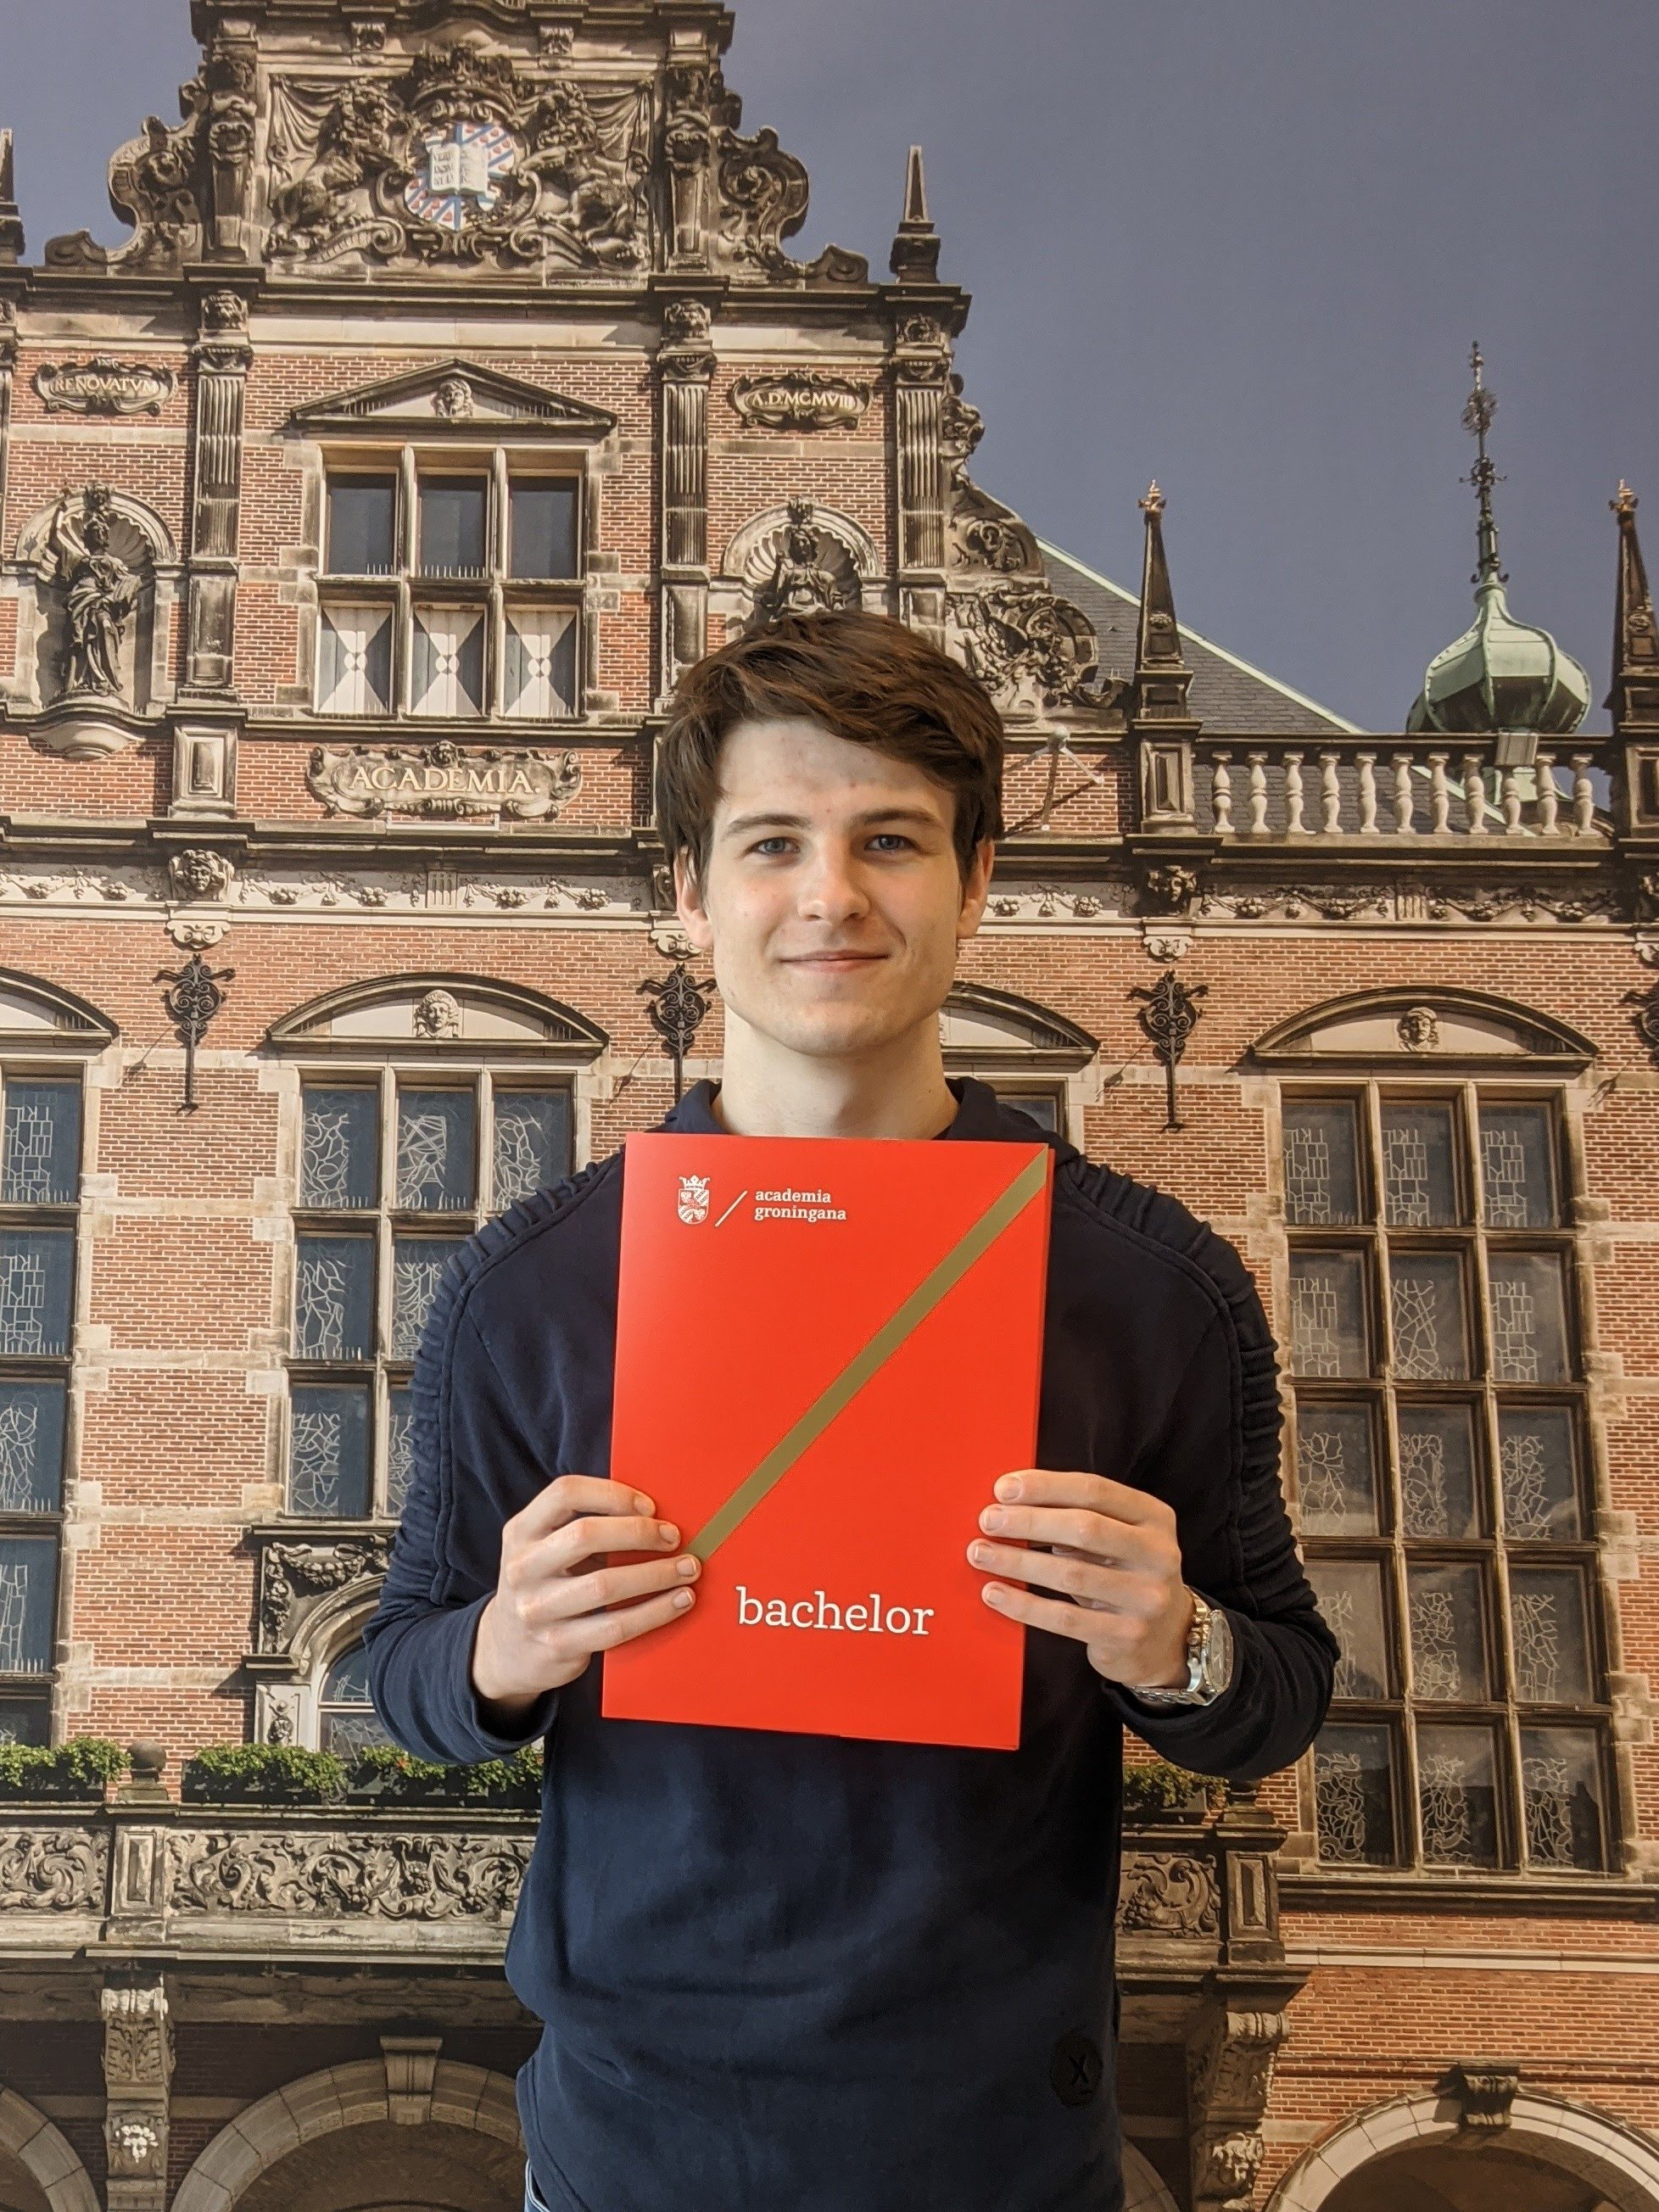
\includegraphics[width=7cm]{profiel_afbeelding.jpg}}; 
        \end{tikzpicture}
    }\\
\end{tabularx}

\sepspace


\section*{Opleidingen}
\hspace{4pt}\begin{tabularx}{\lwmpad}{lXlcr}
    \makecell[tl]{\textbf{\large Master Computing Science}\\\color{darkgray} Rijksuniversiteit Groningen} & & sep. 2020 & ~~-~~ & heden \\
    \rule{0pt}{0.69cm}\makecell[tl]{\textbf{\large Bachelor Computing Science}\\\color{darkgray} Rijksuniversiteit Groningen} & & sep. 2017 & ~~-~~ & jul. 2020 \\
    \rule{0pt}{0.69cm}\makecell[tl]{\textbf{\large Gymnasium}\\\color{darkgray} OSG Sevenwolden, Heerenveen} & & aug. 2011 & ~~-~~ & jul. 2017 \\
\end{tabularx}

\sepspace


\section*{Vaardigheden}
\hspace{4pt}\begin{tabularx}{\lwmpad}{p{\hlwmpad} X p{\hlwmpad}}
% for some reason a tabularx inside another tabularx needs to be enclosed in {}, I don't understand latex well enough to know why :)
    {\begin{tabularx}{\linewidth}[t]{l X r l}
        \adjustbox{valign=t}{\textbf{\large Java}} & & \adjustbox{valign=t}{\skill{4}} & 
        \\
        \rule{0pt}{0.69cm}\adjustbox{valign=t}{\textbf{\large Kotlin}} & & \adjustbox{valign=t}{\skill{4}} & 
        \\
        \rule{0pt}{0.69cm}\adjustbox{valign=t}{\textbf{\large JavaScript}} & & \adjustbox{valign=t}{\skill{4}} & 
        \\
    \end{tabularx}}
    & &
    {\begin{tabularx}{\linewidth}[t]{l X r l}
        \rule{0pt}{0.69cm}\adjustbox{valign=t}{\textbf{\large Python}} & & \adjustbox{valign=t}{\skill{3}} & 
        \\
        \rule{0pt}{0.69cm}\adjustbox{valign=t}{\textbf{\large Docker}} & & \adjustbox{valign=t}{\skill{3}} & 
        \\
    \end{tabularx}}
    \\
\end{tabularx}

\sepspace


\section*{Talen}
\hspace{4pt}\begin{tabularx}{\lwmpad}{p{\hlwmpad} X p{\hlwmpad}}
    \adjustbox{valign=t}{\textbf{\large Nederlands}} \hfill \adjustbox{valign=t}{\skill{5}} & &
    \adjustbox{valign=t}{\color{gray} moedertaal} \\
    % \\
    \rule{0pt}{0.69cm}\adjustbox{valign=t}{\textbf{\large Engels}} \hfill \adjustbox{valign=t}{\skill{5}} & &
    \adjustbox{valign=t}{\color{gray} vloeiend} \\
    % \\
\end{tabularx}



% % Jesse said to make a hybrid of bothe CV's, so more bullet-points but also need adequate description
% \begin{itemize}
%     \item[\heartstab] \textbf{High-school:} Never took German class seriously. To this day I don't speak German. 
%     \item[\squigarr] I think I learned my lesson. I regret not having learned German, I wish I could speak to my German colleagues in their mother tongue now. 
% \end{itemize}

% \sepspace



% %%% Work experience
% %%% ------------------------------------------------------------
% \NewPart{Work Experience}{}

% \begin{itemize}
%     \item[\heartstab] Summer 2021 Rejected from XYZ. 
%     \item[\heartstab] Summer 2021, didn't participate in the final round of the Alibaba math competition. 
%     \item[\heartstab] Spring 2021 University research scholarship, my sloppy last minute application was rejected \squigarr Don't make a last minuet sloppy application. Write multiple drafts days in advance. 
%     \item[\heartstab] DEF, rejected \squigarr they replied and were cordial, and told me they would get back to me if they needed me in the future.
%     \item[\heartstab] Lorum Ipsum rejected me \squigarr twitter DMs work better than cold emails.
% \end{itemize}



% \sepspace

% %%% Skills
% %%% ------------------------------------------------------------
% \NewPart{Skills}{}

% \SkillsEntry{French}{Never really worked on my written french. My reading speed in French is abysmal.}
% \SkillsEntry{German}{Never took German class seriously. My speaking skills are abysmal.}
% \SkillsEntry{Software}{I struggle to get the hang of JS for a long time.}

% %%% Achievements
% %%% -----------------------------------------------------------

% \NewPart{Achievements and Interests}{}

% \begin{itemize}
%     \item[\heartstab] Dropped out of University Club summer 2021 as the team lead. \squigarr Don't bite off more than you can chew. Don't accept something just because you can. 
%     \item[\heartstab] Didn't complete the 2021 DEFG international math competition final round because of self-esteem issues. \squigarr Don't be scared of losing at stuff. Nothing ever comes out of self pity.
%     \item[\heartstab] Never applied to University entrance scholarship \squigarr this would have been good to have, as a credential, and for money, even though the fees are not too dear here it's still easy money. 
%     \item[\heartstab] I haven't played any music in years \squigarr sometimes you need to make sacrifices to get what you want. You can't have everything you want at the same time. Though sad I think it was a good decision. 
% \end{itemize}
    
%\fi


\end{document}


